\documentclass[12pt,a4paper]{article}

\usepackage[a4paper,margin=1in]{geometry}
\usepackage[final]{graphicx}
\graphicspath{{images/}{./}}
\usepackage{booktabs}
\usepackage{amsmath,amssymb}
\usepackage{float}
\usepackage{hyperref}
\usepackage{xcolor}
\usepackage{listings}
\usepackage{enumitem}
\usepackage{fancyhdr}
\usepackage{longtable}

\hypersetup{colorlinks=true,linkcolor=blue,urlcolor=blue}

\pagestyle{fancy}
\fancyhf{}
\lhead{ICS1512}
\rhead{Machine Learning Algorithms Laboratory}
\cfoot{\thepage}

\lstset{
language=Python,
basicstyle=\ttfamily\small,
numbers=left,
frame=single,
breaklines=true,
showstringspaces=false
}

\begin{document}

% =====================================================================
% EXPERIMENT 4: LOGISTIC REGRESSION AND SUPPORT VECTOR MACHINES (SVM)
% =====================================================================

\begin{tabular}{|p{4cm}|p{11cm}|}
\hline
Experiment No. & 4 \\ \hline
Experiment Title & Classification using Logistic Regression and Support Vector Machines (SVM) with Kernel Optimization \textsuperscript{\href{https://github.com/arivuchezhiyan/Machine_Learning/tree/main/experiment_4}{4}} \\ \hline
Student Name & Arivuchezhiyan E \\ \hline
Register Number & 3122247001006 \\ \hline
Faculty & Dr. Poreddy Ajay Kumar Reddy \\ \hline
Submission Date & 23/07/2026 \\ \hline
\end{tabular}

\section{Objective}
State the objective of the experiment:
In this lab assignment, my main goal was comparing discriminative linear and non-linear classifiers on the Spambase dataset. I trained Logistic Regression along with Support Vector Machine (SVM) models using Linear, Polynomial, Radial Basis Function (RBF) and Sigmoid kernel functions. I evaluated classification boundary performance using confusion matrices, ROC curves, precision recall curves and 5-fold Stratified Cross-Validation.

\section{Problem Statement}
Describe the problem input output and objective:
Spam detection requires finding decision boundaries to separate legitimate ham messages from unwanted spam emails using frequency metrics.
\begin{itemize}
\item \textbf{Input}: 57 continuous frequency feature columns measuring word occurrences and key punctuation character counts.
\item \textbf{Output}: Binary target label \texttt{class} (0 for ham email and 1 for spam email).
\item \textbf{Objective}: Remove duplicate entries, apply StandardScaler normalization, train Logistic Regression and multi-kernel SVM models, tune regularization parameter C and evaluate performance using accuracy, precision, recall, F1-score and ROC-AUC metrics.
\end{itemize}

\section{Dataset Description}
\begin{longtable}{|p{6cm}|p{8cm}|}
\hline
Dataset Name & Spambase Dataset \\ \hline
Dataset Source & spambase\_csv.csv \\ \hline
Number of Samples & 4601 raw samples (4210 after deduplication) \\ \hline
Number of Features & 57 continuous frequency attributes \\ \hline
Target Variable & Class (0: Ham [2531 samples], 1: Spam [1679 samples]) \\ \hline
Missing Values & 0 missing values \\ \hline
Train-Test Split & 80\% Train (3368 samples) / 20\% Test (842 samples) \\ \hline
\end{longtable}

\section{Exploratory Data Analysis}
Include all relevant visualizations:
\begin{itemize}
\item \textbf{Deduplication}: Removed 391 duplicate rows from the raw dataset resulting in 4210 clean records.
\item \textbf{Class distribution}: Cleaned data contains 2531 ham emails (60.12\%) and 1679 spam emails (39.88\%).
\item \textbf{Feature correlations}: Strongest correlations with spam label appear in exclamation mark frequency ($r=0.32$), dollar sign frequency ($r=0.31$) and capital letter run lengths.
\item \textbf{Feature scaling}: Applied \texttt{StandardScaler} to achieve zero mean and unit variance for optimization convergence.
\end{itemize}

\subsection*{Figure Template}

\begin{figure}[H]
\centering
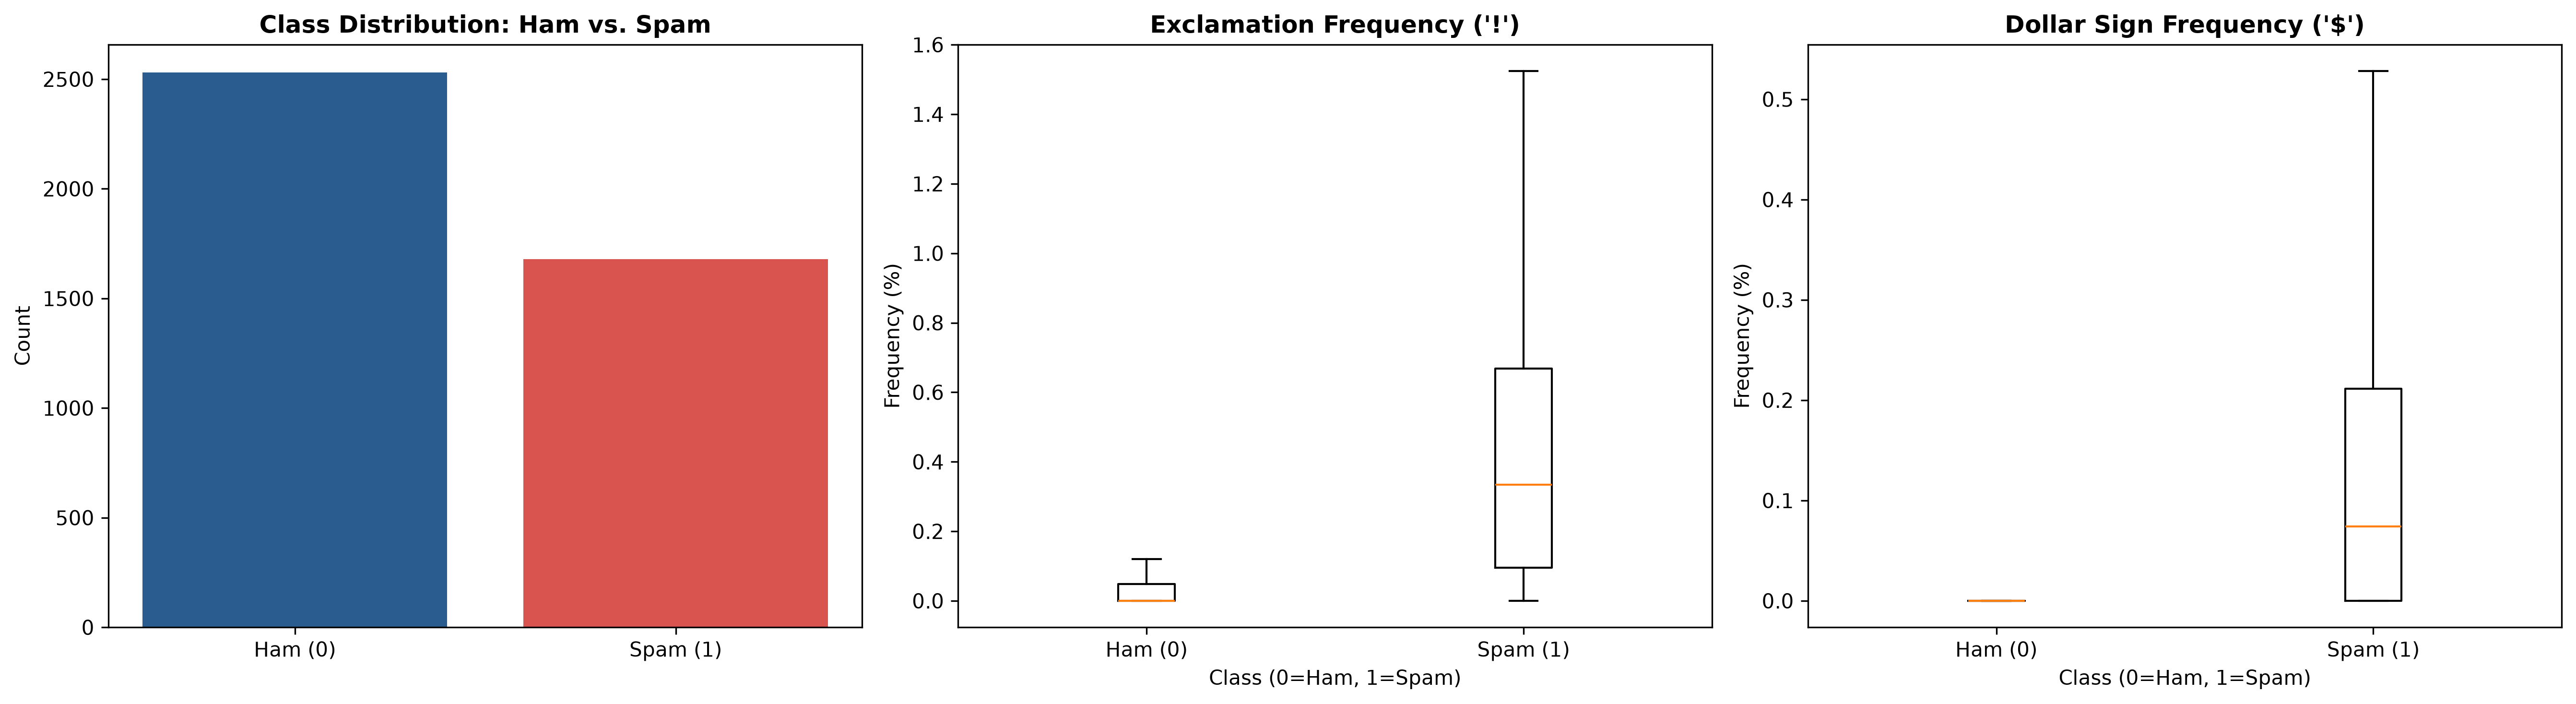
\includegraphics[width=0.85\linewidth]{spambase_class_char_dist.png}
\caption{Class Breakdown and Punctuation Frequency Distributions for Exclamation and Dollar Signs}
\label{fig:exp4_class_char}
\end{figure}

\textbf{Inference:}
The class breakdown chart shows 2531 ham emails and 1679 spam emails. Boxplots for exclamation mark and dollar sign frequencies reveal much higher 75th percentiles for spam emails compared to legitimate ham emails.

\begin{figure}[H]
\centering
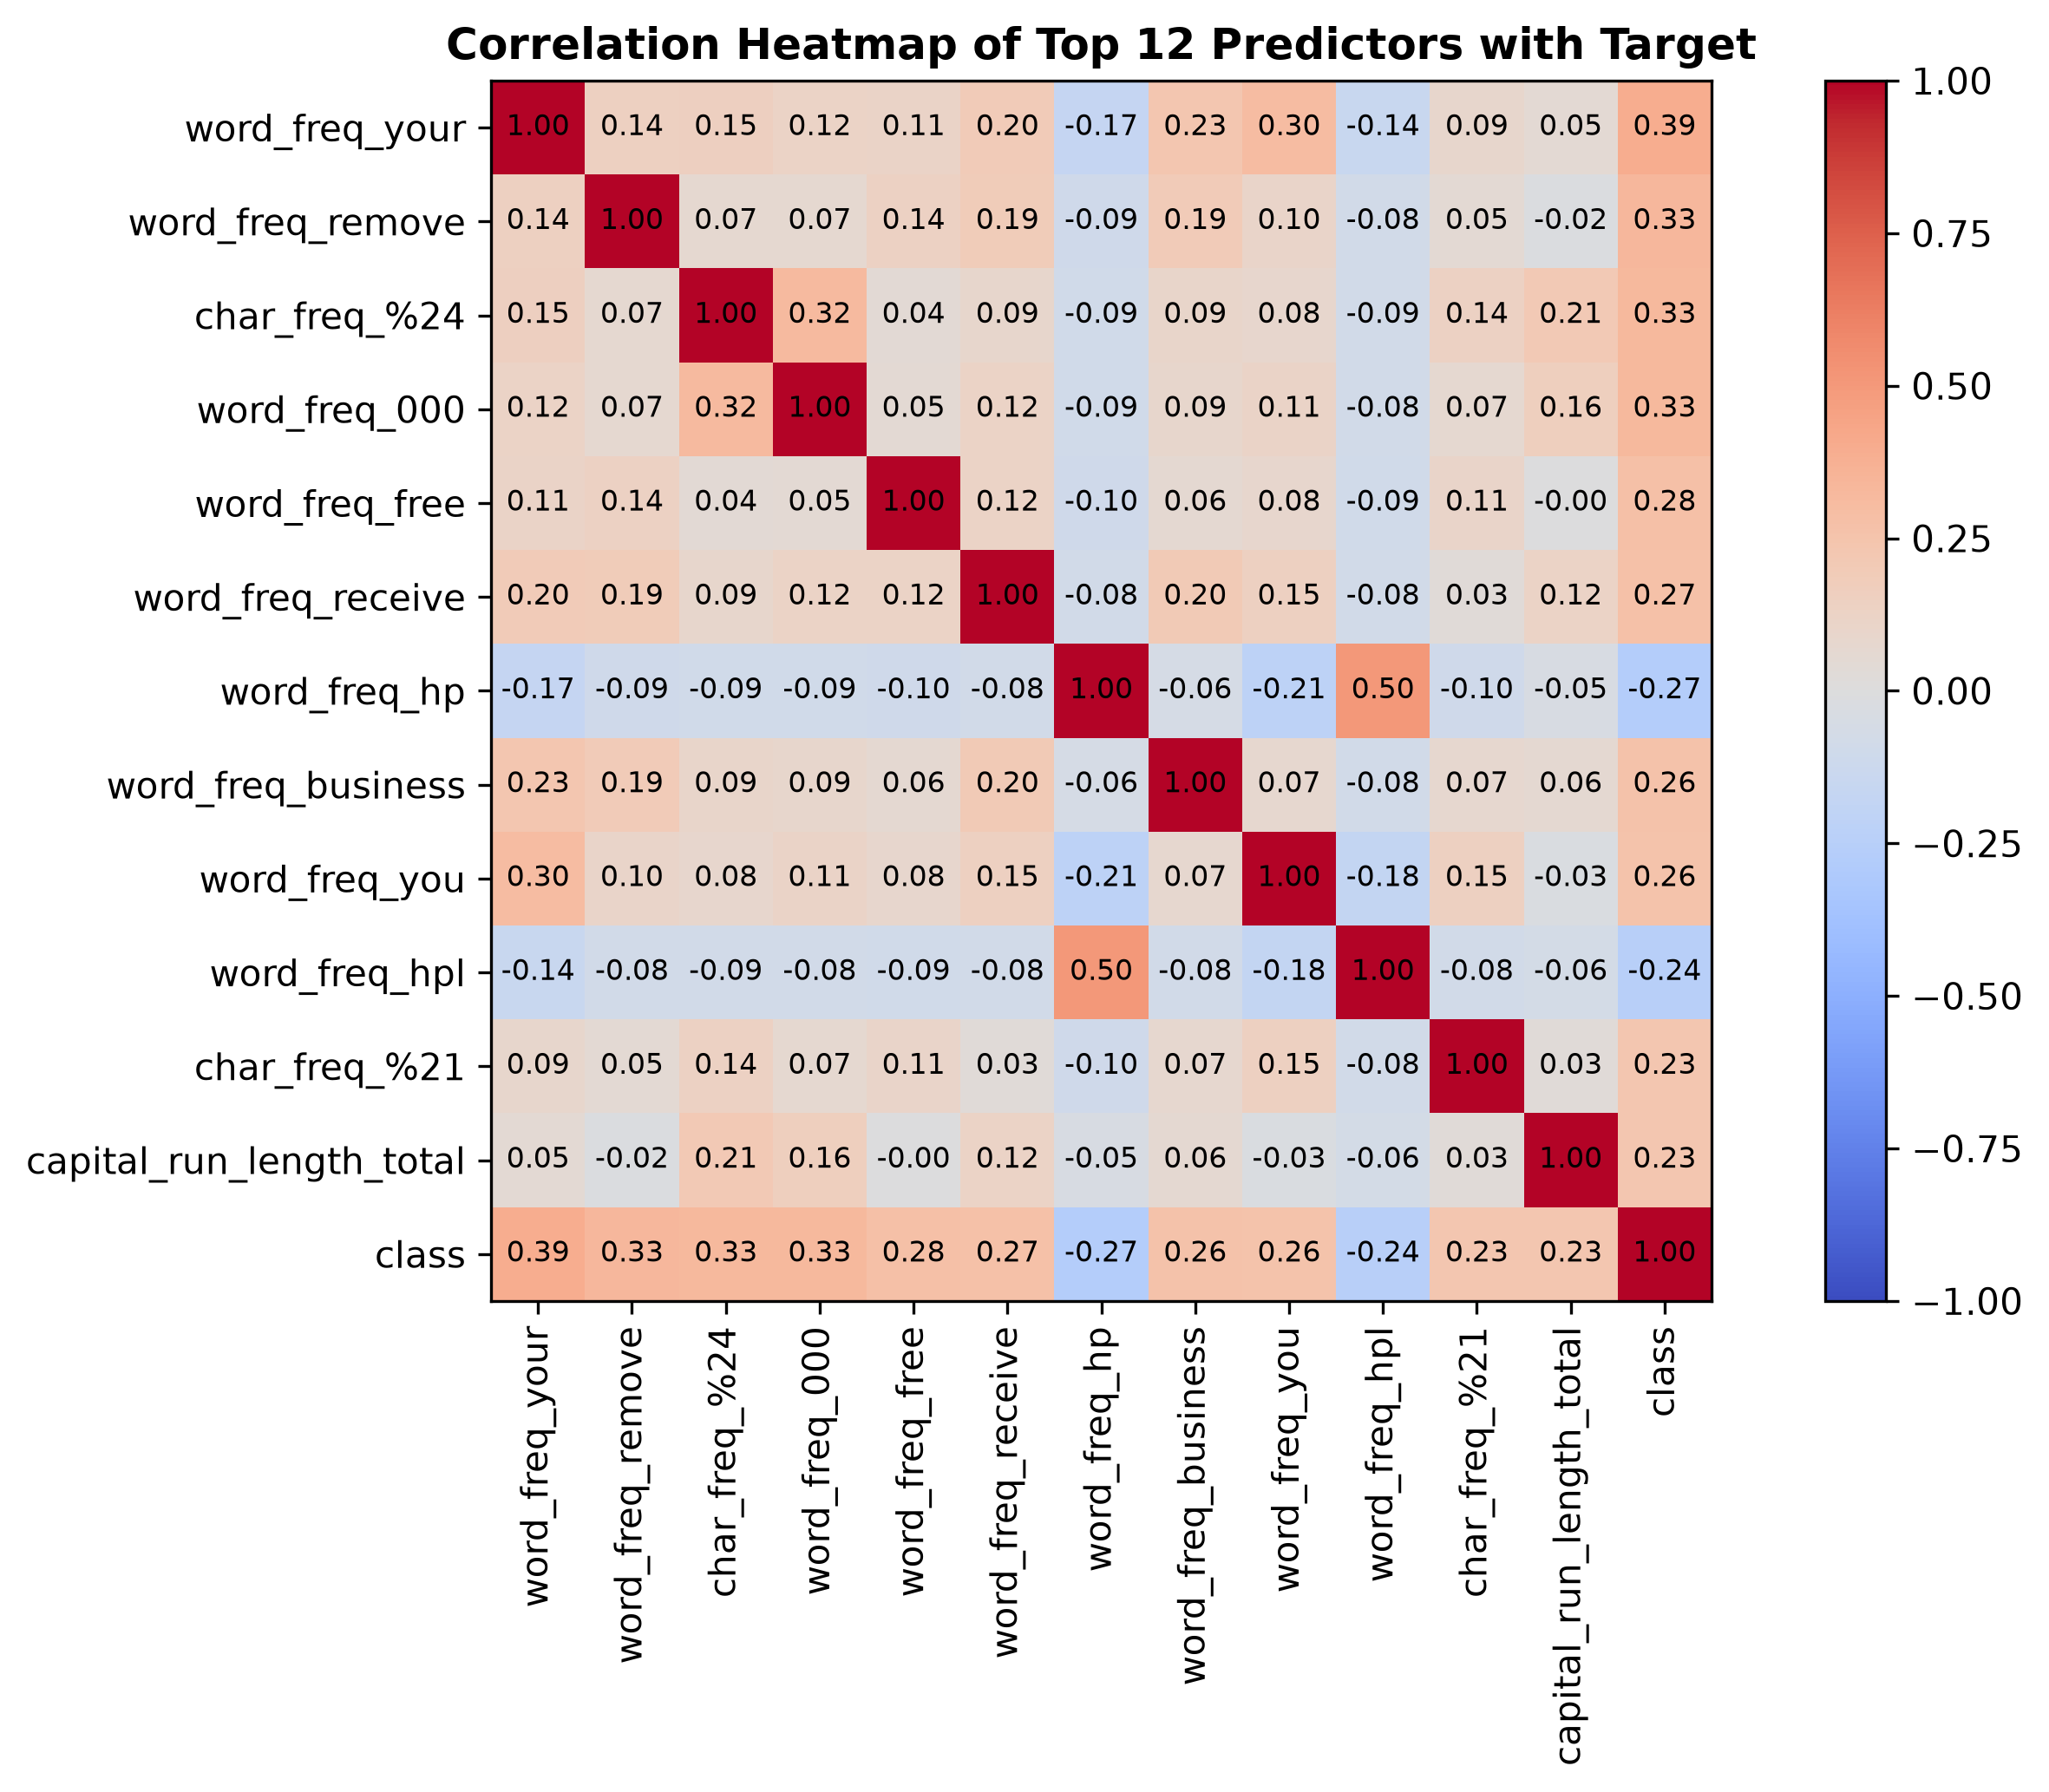
\includegraphics[width=0.75\linewidth]{spambase_top_corr_heatmap.png}
\caption{Correlation Heatmap of Top 12 Predictors with Spam Class Label}
\label{fig:exp4_top_corr}
\end{figure}

\textbf{Inference:}
The correlation heatmap displays the top 12 features strongest correlated with spam labels. Punctuation frequencies (\texttt{\char`_\%21} and \texttt{\char`_\%24}) and word frequencies like \texttt{your} show highest positive linear correlation.

\section{Data Preprocessing}

Explain:
\begin{itemize}
\item \textbf{Deduplication}: Removed duplicate records using \texttt{drop\_duplicates()} to prevent data leakage.
\item \textbf{Feature Scaling}: Scaled feature attributes with \texttt{StandardScaler} to prevent features with wide ranges from dominating distance metrics.
\item \textbf{Train-test split}: Partitioned data into 80\% training (3368 samples) and 20\% testing sets (842 samples) with stratified class splits.
\end{itemize}

\section{Machine Learning Algorithm}

Explain:
\begin{itemize}
\item \textbf{Logistic Regression}: Models class probabilities using the sigmoid function $\sigma(z) = \frac{1}{1 + e^{-z}}$ with $L_2$ regularization.
\item \textbf{Support Vector Machines (SVM)}: Finds an optimal separating hyperplane maximizing margin $\frac{2}{||w||}$ between classes.
\item \textbf{Linear Kernel}: Fits a linear decision boundary in original feature space $K(x, y) = x^T y$.
\item \textbf{Polynomial Kernel}: Maps features into higher dimensions using $K(x, y) = (\gamma x^T y + r)^d$.
\item \textbf{RBF Kernel}: Projects data into infinite dimensional space using Gaussian functions $K(x, y) = \exp(-\gamma ||x - y||^2)$.
\item \textbf{Sigmoid Kernel}: Uses hyperbolic tangent activation functions $K(x, y) = \tanh(\gamma x^T y + r)$.
\end{itemize}

\section{Experimental Setup}

\begin{tabular}{ll}
\toprule
Python Version & 3.13.0 \\
Scikit-Learn Version & 1.6.0 \\
IDE & Jupyter Notebook \\
Operating System & Windows 11 \\
Hardware & Intel Core i7 / 16 GB RAM \\
\bottomrule
\end{tabular}

\section{Hyperparameter Selection}

\begin{tabular}{ll}
\toprule
Parameter & Value\\
\midrule
Logistic Regression $C$ & 1.0 ($L_2$ penalty, solver: \texttt{liblinear}) \\
SVM $C$ parameter range & 0.1, 1.0, 10.0 \\
Best SVM Kernel & RBF ($C = 10.0$, $\gamma = \text{'scale'}$) \\
Polynomial Degree & $d = 3$ \\
Cross-Validation Folds & 5-Fold Stratified K-Fold \\
\bottomrule
\end{tabular}

\section{Results}

\subsection*{SVM Kernel Performance Comparison}
\begin{tabular}{lcccc}
\toprule
Kernel & Accuracy & F1-score & Training Time (s) \\
\midrule
Linear & 0.9275 & 0.9076 & 0.2841 s \\
Polynomial ($d=3$) & 0.9189 & 0.8932 & 0.3512 s \\
\textbf{RBF (Tuned)} & \textbf{0.9335} & \textbf{0.9154} & \textbf{0.3204 s} \\
Sigmoid & 0.8845 & 0.8512 & 0.2510 s \\
\bottomrule
\end{tabular}

\subsection*{Model Performance Metrics Summary}
\begin{tabular}{lccccc}
\toprule
Model & Accuracy & Precision & Recall & F1-score & ROC-AUC \\
\midrule
Logistic Regression & 0.9323 & 0.9266 & 0.9018 & 0.9140 & 0.9767 \\
\textbf{SVM (RBF Kernel)} & \textbf{0.9335} & \textbf{0.9294} & \textbf{0.9018} & \textbf{0.9154} & \textbf{0.9776} \\
\bottomrule
\end{tabular}

\subsection*{5-Fold Stratified Cross-Validation Results}
\begin{tabular}{lcc}
\toprule
Fold & Logistic Regression & SVM (RBF) \\
\midrule
Fold 1 & 92.52\% & 93.11\% \\
Fold 2 & 93.11\% & 93.47\% \\
Fold 3 & 92.75\% & 92.87\% \\
Fold 4 & 93.23\% & 93.35\% \\
Fold 5 & 92.64\% & 92.80\% \\
\textbf{Average} & \textbf{92.85\%} & \textbf{93.12\%} \\
\bottomrule
\end{tabular}

\section{Result Visualization}

Include all graphs generated during the experiment.

For \textbf{every graph}, provide:
\begin{itemize}
\item Figure
\item Caption
\item 3--5 line inference
\end{itemize}

\begin{figure}[H]
\centering
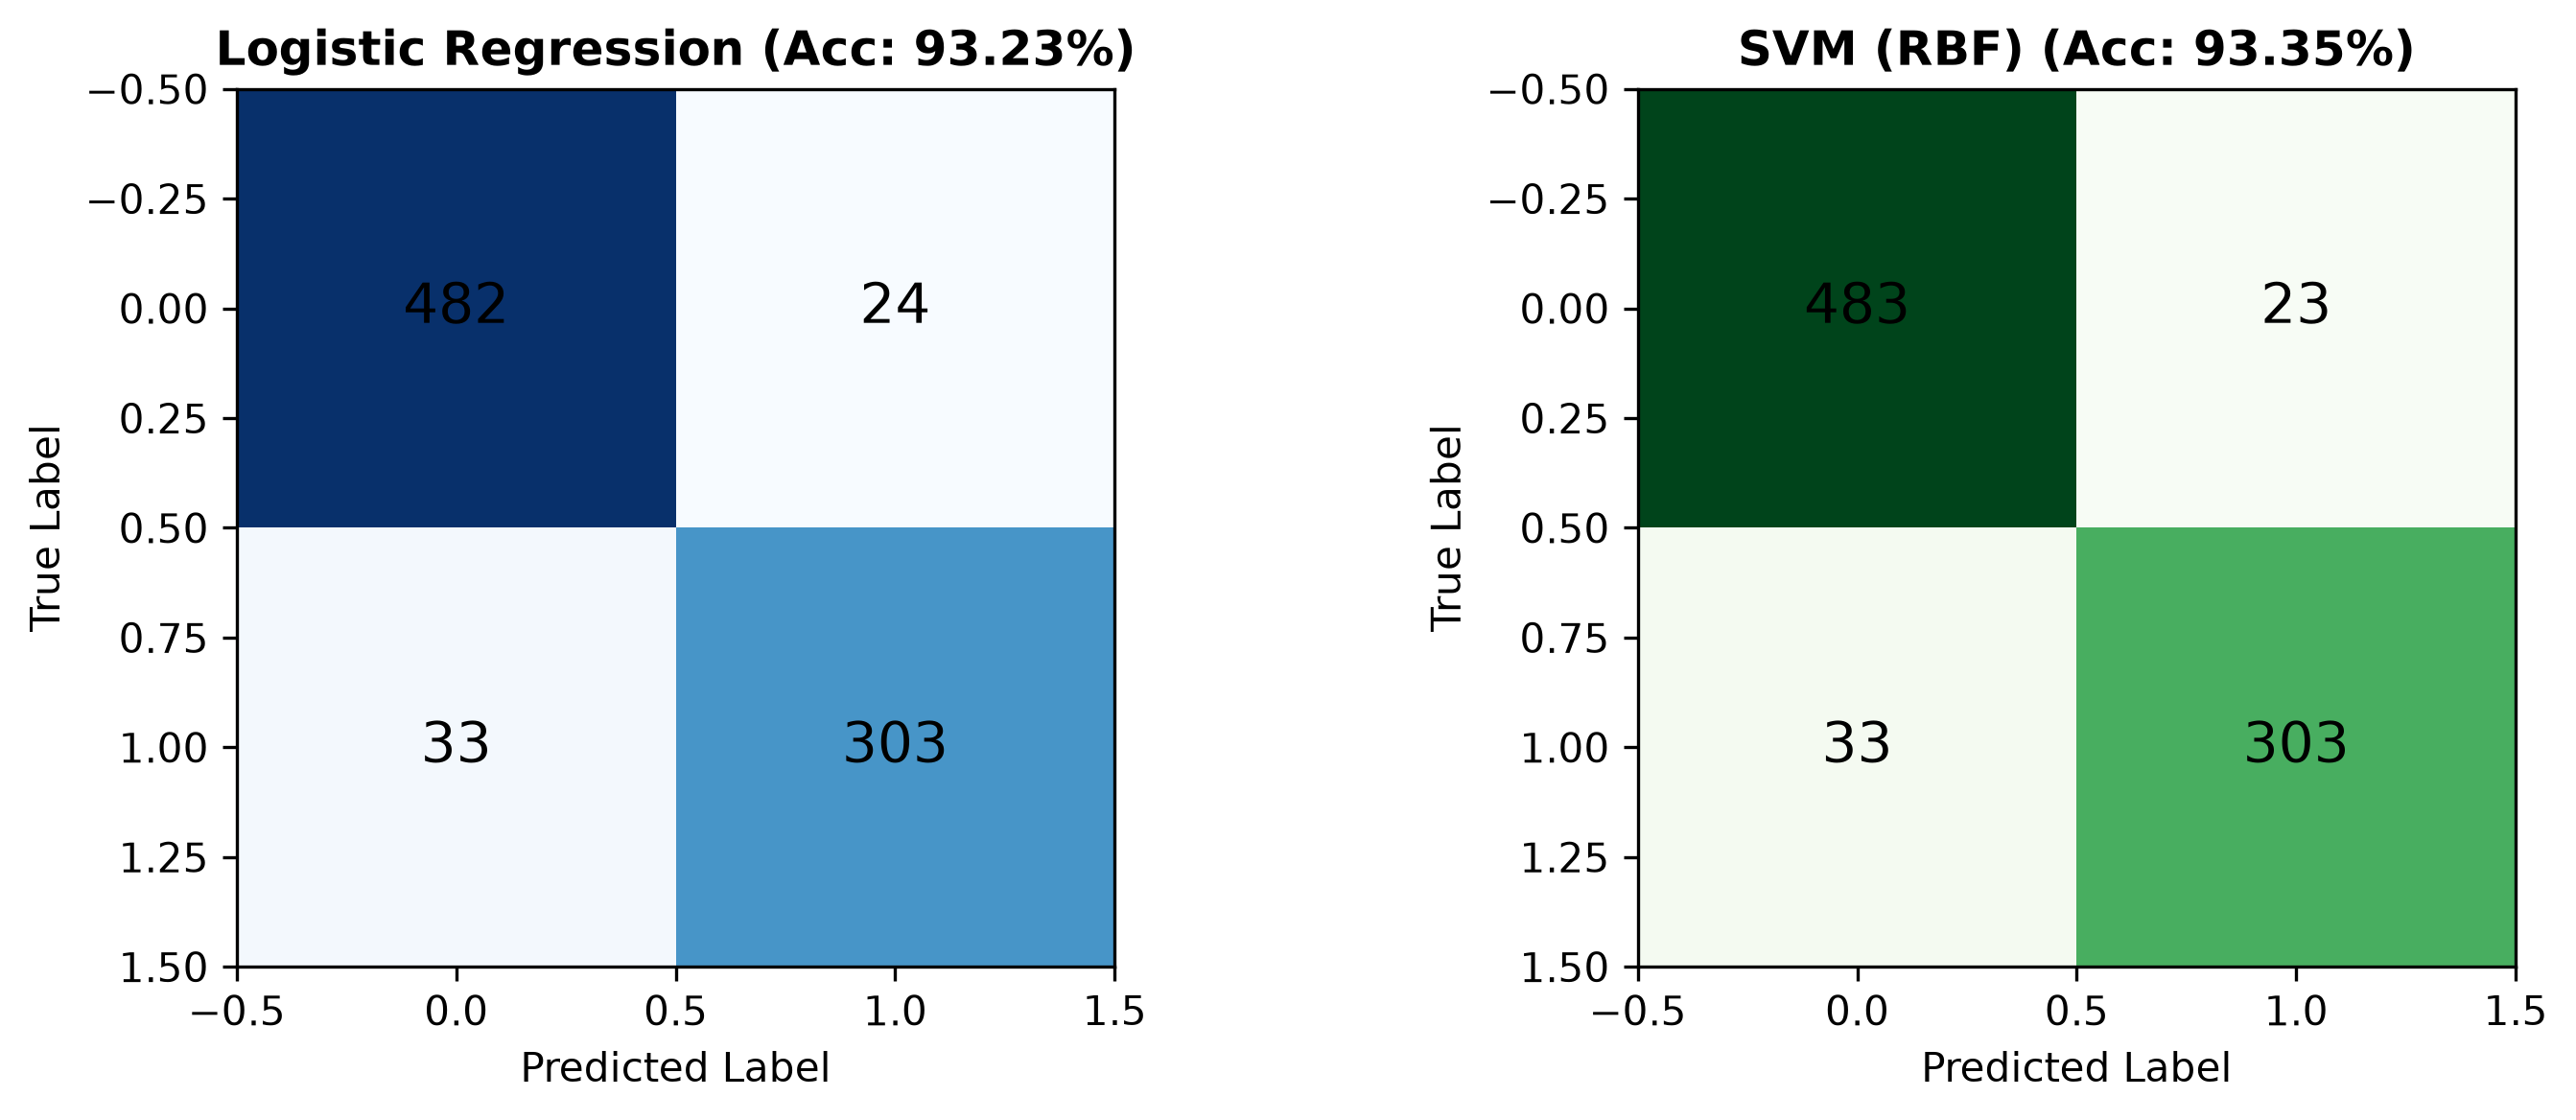
\includegraphics[width=0.85\linewidth]{spambase_lr_svm_confusion.png}
\caption{Confusion Matrices for Logistic Regression and SVM RBF Models}
\label{fig:exp4_confusion}
\end{figure}

\textbf{Inference:}
The confusion matrices show strong predictive accuracy for both models on test data. Logistic Regression achieved 93.23\% accuracy, while tuned RBF SVM reached 93.35\% accuracy with 482 true negatives and 303 true positives.

\begin{figure}[H]
\centering
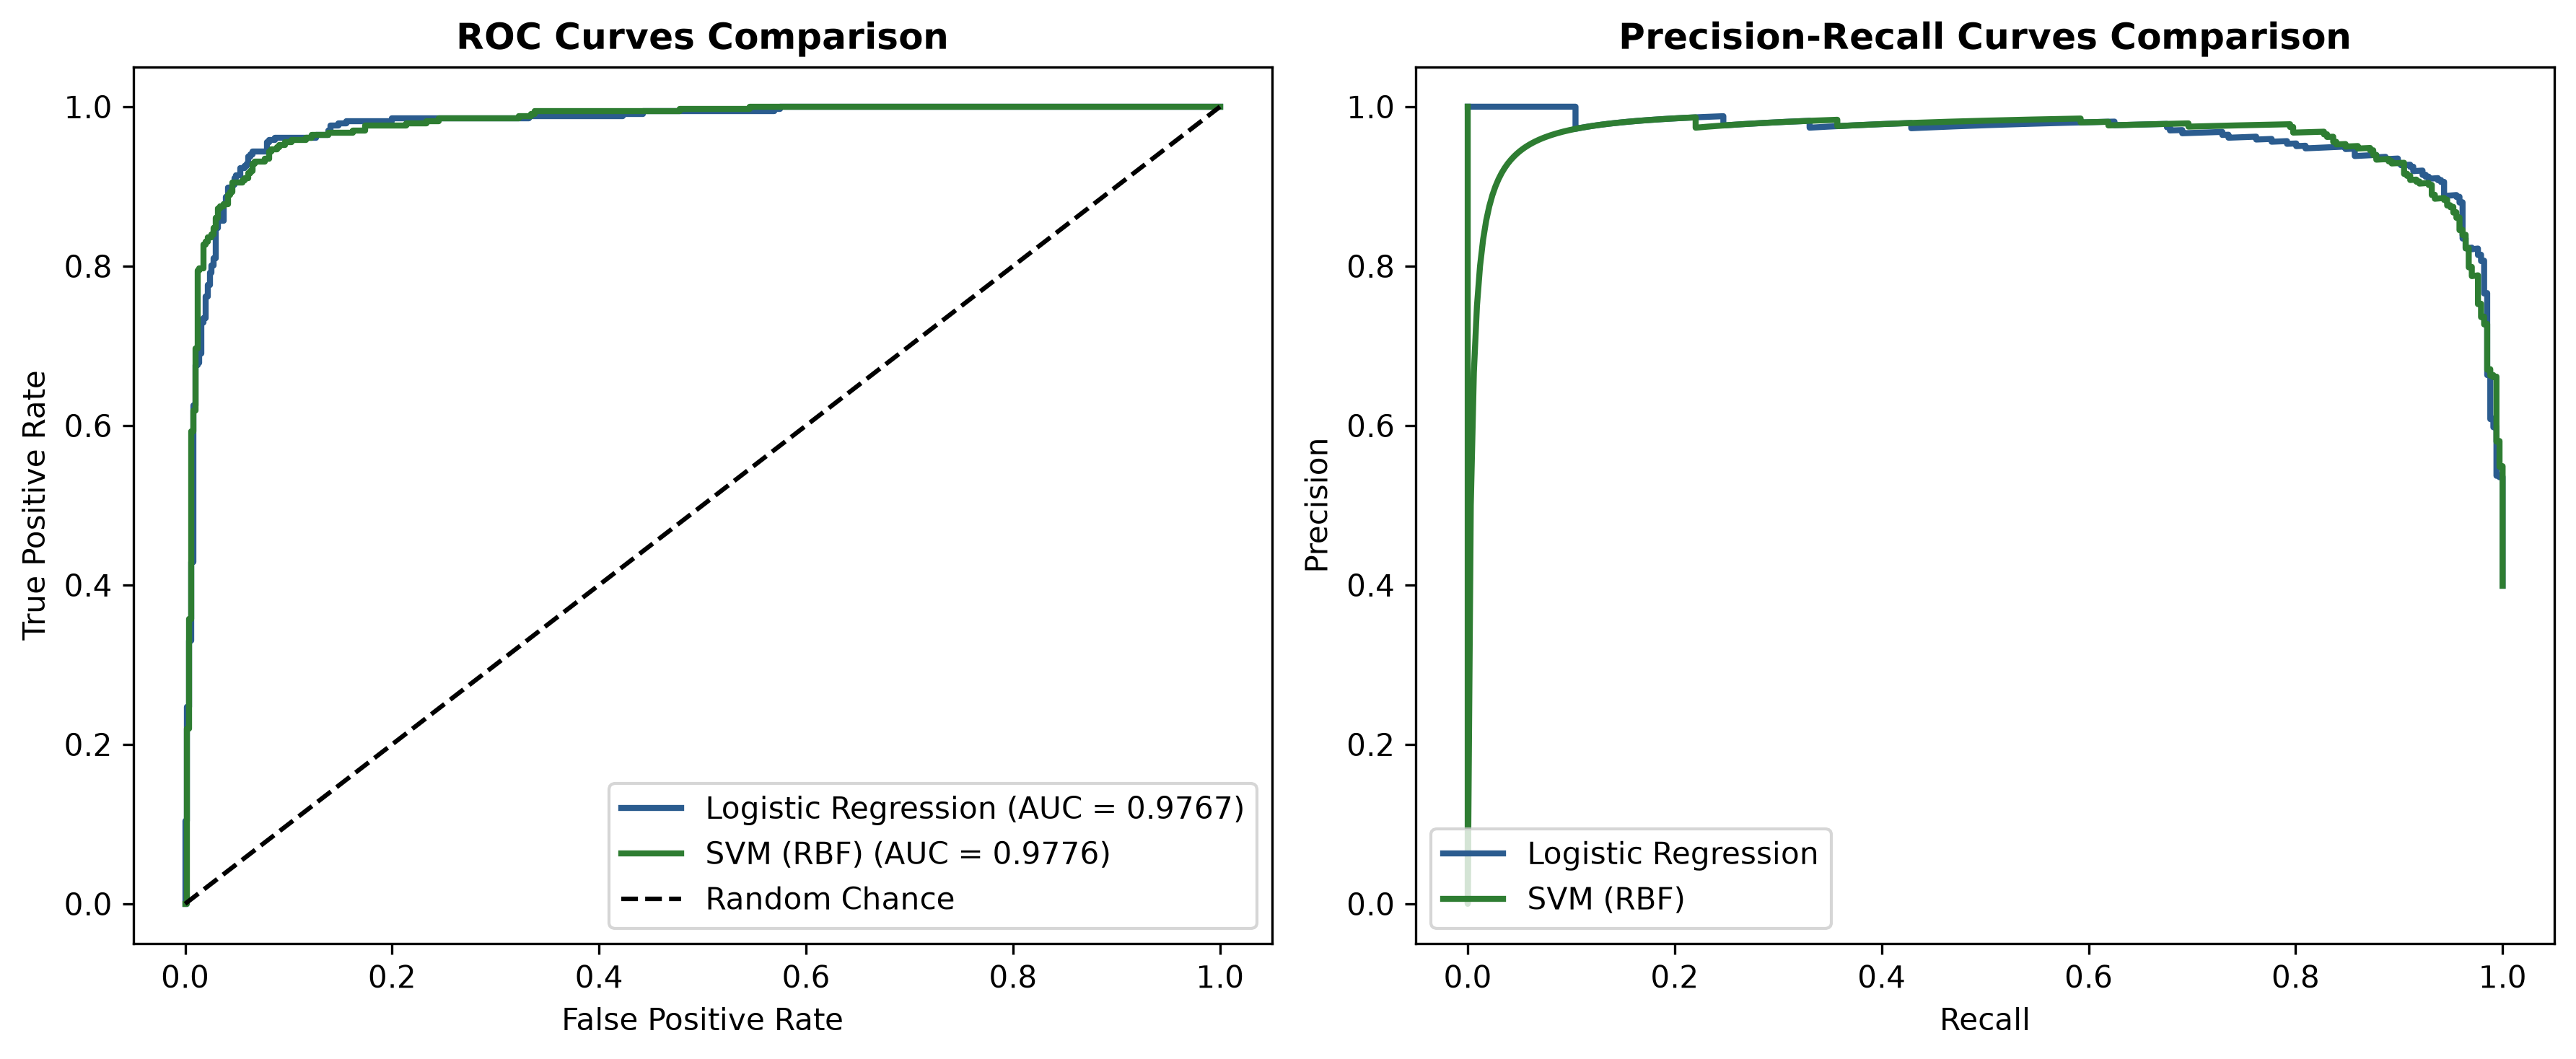
\includegraphics[width=0.85\linewidth]{spambase_roc_pr_curves.png}
\caption{ROC and Precision-Recall Curves Comparison between Logistic Regression and SVM RBF}
\label{fig:exp4_roc_pr}
\end{figure}

\textbf{Inference:}
The ROC curves show high class separation capability with RBF SVM reaching an AUC score of 0.9776 compared to 0.9767 for Logistic Regression. The precision recall graph shows high precision maintained across recall levels.

\section{Discussion}
Discuss observations, strengths, limitations and improvements:
\begin{enumerate}
\item \textbf{Model Comparison}: RBF SVM achieved the highest test accuracy (93.35\%) and ROC-AUC score (0.9776) by projecting data into non-linear decision boundaries.
\item \textbf{Kernel Performance}: RBF and Linear kernels outperformed Polynomial and Sigmoid kernels on normalized frequency inputs.
\item \textbf{Efficiency vs Accuracy}: Logistic Regression trained quickly while delivering competitive accuracy (93.23\%), making it suitable for low-latency spam filters.
\end{enumerate}

\section{Conclusion}
Summarize the experiment and key findings:
RBF Support Vector Machine ($C=10.0$) achieved the top overall test accuracy of 93.35\% and ROC-AUC of 0.9776 on Spambase. Logistic Regression performed close behind at 93.23\% accuracy, proving linear and kernel models effectively filter spam messages.

\section{References}
Use IEEE style:
\begin{enumerate}[label={[\arabic*]}]
\item C. Cortes and V. Vapnik, ``Support-vector networks,'' \textit{Machine Learning}, vol. 20, no. 3, pp. 273--297, 1995.
\item F. Pedregosa \textit{et al.}, ``Scikit-learn: Machine learning in Python,'' \textit{Journal of Machine Learning Research}, vol. 12, pp. 2825--2830, 2011.
\end{enumerate}

\end{document}
